\documentclass{article}

\usepackage{tikz}

\tikzset{
    treenode/.style = {
        shape=circle,
        draw,
        align=center,
        top color=white,
        bottom color=blue},
    root/.style = {
        treenode,
        font=\Large,
        bottom color=red},
    env/.style = {
        treenode,
        font=\ttfamily\normalsize},
    dummy/.style = {
        circle,
        draw}
}


\begin{document}

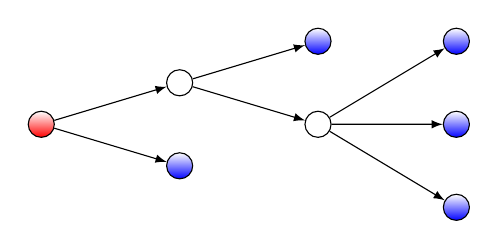
\begin{tikzpicture}[
    grow                    = right,
    sibling distance        = 3em,
    level distance          = 5em,
    edge from parent/.style = {draw, -latex},
    every node/.style       = {font=\footnotesize},
    sloped
]

\node [root] {}
    child { node [env] {}
        edge from parent node {}}
    child { node [dummy] {}
        child { node [dummy] {}
            child { node [env] {}
                edge from parent node {}}
            child { node [env] {}
                edge from parent node {}}
            child { node [env] {}
                edge from parent node {}}
            edge from parent node {}}
        child { node [env] {}
            edge from parent node {}}
        edge from parent node {}};

\end{tikzpicture}
\end{document}

